\documentclass[
  ngerman,
  DIV=14
]{scrartcl}
\usepackage{babel}
\usepackage{csquotes}

% typography
\usepackage{fontspec}
\usepackage[utopia]{mathdesign}
\setsansfont{Open Sans}[
  BoldFont={Open Sans Bold},
  ItalicFont={Open Sans Italic}]
\setmonofont[Scale=0.85]{Menlo}
\setmainfont{Palatino}
\linespread{1.15}
%\renewcommand\familydefault{\sfdefault}
\usepackage[factor=2000]{microtype}

% graphics, drawings, etc.
\usepackage{xcolor}
\usepackage{graphicx}
\usepackage[most]{tcolorbox}
\usepackage{tikz}
\usetikzlibrary{shapes.geometric}
\usetikzlibrary{shapes.arrows}
\usetikzlibrary{positioning}
\newtcolorbox{anmerkung}{%
  grow to left by=10pt,
  colback=black!10,
  colframe=white,
  coltitle=black,
  borderline west={4pt}{0pt}{black!30},
  boxrule=0pt,
  boxsep=0pt,
  %breakable,
  enhanced jigsaw,
  title={Anmerkung\par},
  fonttitle={\bfseries},
  attach title to upper={}}
\newtcolorbox{hinweis}{%
  grow to left by=10pt,
  colback=black!10,
  colframe=white,
  coltitle=black,
  borderline west={4pt}{0pt}{black!30},
  boxrule=0pt,
  boxsep=0pt,
  %breakable,
  enhanced jigsaw,
  title={Hinweis\par},
  fonttitle={\bfseries},
  attach title to upper={}}

% highlighting, lists, code
\usepackage{soul}
\usepackage{enumitem}
\usepackage{listings}
\lstset{
  basicstyle=\ttfamily,
  %escapeinside=||,
  keywordstyle=\color{blue!50!black},
  stringstyle=\color{green!50!black}}
\capsdef{////}{\scshape}{.16em}{.4em}{.2em}

% math
\usepackage{amsmath}

% nice tables
\usepackage{booktabs}
\newcommand{\tablespacing}[1]{\renewcommand{\arraystretch}{#1}}

% links
\usepackage[
  colorlinks,
  linkcolor={red!50!black},
  citecolor={blue!50!black},
  urlcolor={blue!80!black}
]{hyperref}

\title{Lösungsblatt Nr. 1}
\date{Wintersemester 2018-2019}
\author{Andreas Koch}
\subject{Einführung in den Compilerbau}
\subtitle{Patrick Elsen, Viola Hofmeister und Michael Matthé}
\publishers{Technische Universität Darmstadt}

\begin{document}
\maketitle

\subsection*{Einleitung}

Auf diesem Aufgabenblatt sollen Sie sich mit der Matrix and Vector Language, kurz MAVL, vertraut machen. Studieren Sie bitte zunächst die MAVL-Sprachspezifikation, die Sie im Moodle-Kurs der Veranstaltung finden.

\subsection*{Aufgabe 1.1: MAVL-Syntax}

Die MAVL-Sprachspezifikation enthält nur eine informelle Beschreibung der Syntaxelemente der Sprache. In den folgenden Teilaufgaben sollen Sie einige der Syntaxelemente in Produktionen einer kontextfreien Grammatik überführen.

\subsection*{Aufgabe 1.1a: Produktionen}

Geben Sie Produktionen für die Nichtterminale \texttt{mulExpr} (Multiplikations-Operator), \texttt{subvectorExpr} (Subvektor-Operator), sowie \texttt{recordElementSelectExpr} (Selektion von Record-Elementen) an.

\bigskip\noindent
Ein Multiplikationsausdruck ist in der Sprachspezifikation unter \emph{§~7.5 Ternärer Operator} definiert. Ein solcher Ausdruck nimmt \verb|int| oder \verb|float|-Ausdrücke als Parameter und ist Linksassoziativ. Also kann man diesen grammatikalisch folgendermaßen definieren. 
\begin{verbatim}
mulExpr ::= expr '*' expr
\end{verbatim}
Die \verb|subvectorExpr| ist in dem Sprachstandard unter \emph{§~7.7.4 Submatrix und Subvektor} definiert. Hier wird definiert, dass eine solche Beispielsweise als \verb|v{-1:i:1}| geschrieben werden kann, wobei \verb|v| ein Vektor und \verb|i| eine Zahl sein muss. Dieser Ausdruck extrahiert einen Subvektor mit den Elementen $[i-1, i+1]$. Der Vektor kann also eine ID sein, oder ein anderer Ausdruck, der einen Vektor zurückgibt. Also nehmen wir \texttt{expr}. In dem Subvektorausdruck selbst kann der mittlere Term ein beliebiger Ausdruck sein, die ersten beiden Terme aber müssen konstante Ausdrücke sein. Das bedeutet, dass diese sich nur aus Zahlen (mit Vorzeichen) und Operatoren bestehen dürfen. Um die Grammatik kompakt zu beschreiben, wird auf diese Einschränkung verzichtet und wir nehmen auch hier \texttt{expr}.
\begin{verbatim}
subvectorExpr ::= expr '{' expr ':' expr ':' expr '}'  
\end{verbatim}
Unter \emph{§~7.8 Selektion von Record-Elementen} ist definiert, wie der Syntax funktioniert. Hier kann man aus einem Ausdruck, der eine Instanz eines Record darstellt, auf ein einzelnes Element zugreifen. Mit dem Ausdruck \texttt{person@name} greift man zum Beispiel auf das Namenselement einer Person zu. 
\begin{verbatim}
recordElementSelectExpr ::= expr '@' ID  
\end{verbatim}

\subsection*{Aufgabe 1.1b}

Geben Sie Produktionen für die Nichtterminale \verb|primitiveType| (primitive Typen) und \verb|vectorType| (Vektortypen) an.

\bigskip\noindent
Die primitiven Typen sind unter \emph{§~4.2 Primitive Datentypen} definiert. Hier sind nur \texttt{int}, \texttt{float} und \texttt{bool} als eingebaute, primitive Typen angegeben. Also könnte eine Grammatik folgendermaßen aussehen:
\begin{verbatim}
primitiveType ::= 'int' | 'float' | 'bool'
\end{verbatim}
Der \texttt{vectorType} ist bei \emph{§~4.5 Vektoren} definiert. Ein Vektor muss, mit einem Elementtyp (entweder \texttt{int} oder \texttt{float}) und einer Länge (positive, ganze Zahl) definiert werden.
\begin{verbatim}
vectorType ::= 'vector' '<' ('int' | 'float') '>' '[' expr ']'
\end{verbatim}

\subsection*{Aufgabe 1.1c}

Geben Sie Produktionen für die Nichtterminale \texttt{returnStmt} (Rückgabebefehl), \texttt{varDecl} Variablendeklaration), \texttt{callStmt} (Aufruf-Befehl, ohne Rückgabewert) sowie \texttt{forStmt} (For-Schleife) an.

\bigskip\noindent
Der Rückgabebefehl ist unter \emph{§~6.8 Rückgabe} im Sprachstandard definiert. Ein solcher Befehl besteht aus dem Keyword \texttt{'return'}, einem Ausdruck und einem abschließenden Semikolon. Also kann man einen solchen folgendermaßen definieren.
\begin{lstlisting}
returnStmt ::= 'return' expr ';'
\end{lstlisting}


\subsection*{Aufgabe 1.2: AST zu MAVL}
Abstrakte Syntaxbäume (engl. \emph{Abstract Syntax Tree}) sind eine weitverbreitete Zwischendarstellung, die nur essentielle Informationen enthält und Details der konkreten Syntax einer Programmiersprache abstrahiert. In dieser Aufgabe zeigen wie Ihnen eine mögliche Repräsentation von MAVL-Code als AST. Die darin verwendeten AST-Knoten korrespondieren auf natürliche Weise mit den in der Spezifikation beschriebenen Syntaxelementen. 

\subsection*{Artikel 1.2a}
Geben Sie den zum folgenden AST zugehörigen MAVL-Code an.  

\bigskip\noindent
Den Syntaxbaum kann man, von oben nach unten und links nach rechts, einfach wie Code lesen.
\begin{lstlisting}
if(id && r > q) {
  r = -1;
  q(q, r);
} else {
  r = a - (q * d);
}
\end{lstlisting}


\subsection*{Artikel 1.2b}
Geben Sie den zum folgenden AST zugehörigen MAVL-Code an.  

\bigskip\noindent
\begin{lstlisting}
var vector<int>[3 + 1] p;
for(var int i : p) {
  i = k;
}  
\end{lstlisting}


\subsection*{Artikel 1.3: Ausdrücke}
Ausdrücke in typischen Programmiersprachen lassen sich einfach durch mehrdeutige Grammatiken beschreiben, die aber als Grundlage für die syntaktische Analyse ungeeignet sind.

\subsection*{Artikel 1.3a}
Zeichnen Sie den AST für den MAVL-Ausdruck \texttt{q \& a == b \# c}.


\bigskip\noindent
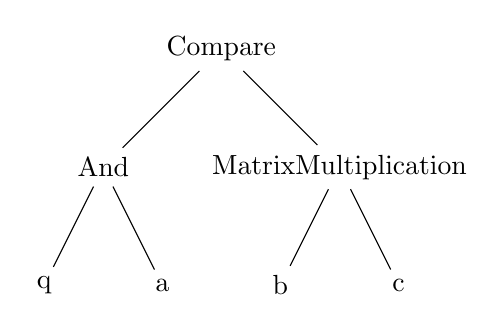
\begin{tikzpicture}[level distance=1.5cm,
level 1/.style={sibling distance=3cm},
level 2/.style={sibling distance=1.5cm}
]
\node{Compare}
child {node {And}
	child {node {q}}
	child {node {a}}
}
child {node {MatrixMultiplication}
	child {node {b}}
	child {node {c}}
};
\end{tikzpicture}


\subsection*{Artikel 1.3b}
Zeichnen Sie den AST für den MAVL-Ausdruck\texttt{ - v2 .* v1 + (v2 \# m)[0]}.


\bigskip\noindent
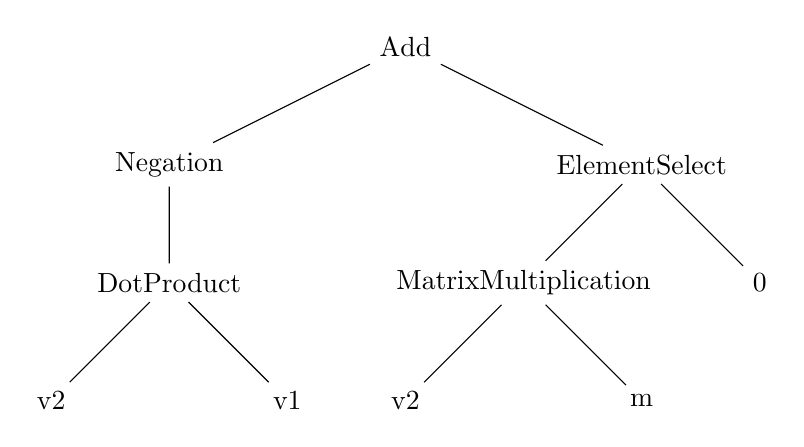
\begin{tikzpicture}[level distance=1.5cm,
level 1/.style={sibling distance=6cm},
level 2/.style={sibling distance=3cm}
]
\node{Add}
child {node {Negation}
	child {node {DotProduct}
		child {node {v2}}
		child {node {v1}}		
	}
}
child {node {ElementSelect}
	child {node {MatrixMultiplication}
		child {node {v2}}
		child {node {m}}
	}
	child {node {0}}
};

\end{tikzpicture}

\subsection*{Aufgabe 1.3c}
Gegeben seien folgende Wertedefinitionen.
\begin{lstlisting}
val matrix <int>[2][2] m = [[1, 2],
                            [3, 4]];
val vector<int>[2]    v1 = [4, 2];
val vector<int>[2]    v2 = [2, 3];
\end{lstlisting}
Welchen Wert liefert der Ausdruck aus Teilaufgabe 1.3b?

\bigskip\noindent
Antwort.

\end{document}